\documentclass[]{scrreprt}
\usepackage{amsmath,amsfonts,graphicx}
\usepackage{multirow}
\usepackage{pslatex}
\usepackage{tabularx}
\usepackage{comment}
\usepackage{xspace}
\usepackage{array}

\usepackage{hyperref}

\usepackage{caption}
\DeclareCaptionFont{white}{\color{white}}
\DeclareCaptionFormat{listing}{\colorbox{gray}{\parbox{\textwidth}{#1#2#3}}}

\graphicspath{
{figures/}
}

\def\species{\mathrm{sp}}
\def\phase{\beta}
\def\massfrac{\chi}
\def\flux{\mathbf{F}}
\def\darcyvel{\mathbf{v}}
\def\energydens{\mathcal{E}}
\def\d{\mathrm{d}}
\def\diag{\mathrm{diag}\,}

\newcommand{\uo}{\mbox{UO\textsubscript{2}}\xspace}

\setcounter{secnumdepth}{3}


\begin{document}


\title{Heat-Conduction Tests}
\author{CSIRO}
\maketitle

\tableofcontents

\chapter{Simple heat conduction in 1D}

PorousFlow heat conduction is governed by the equation
\begin{equation}
0 = \frac{\partial}{\partial t}\energydens + \nabla\cdot \flux^{\mathrm{T}} \ ,
\label{eqn.heat.cond}
\end{equation}
Here $\energydens$ is the energy per unit volume in the rock-fluid
system, and $\flux^{\mathrm{T}}$ is the heat flux.  In the
PorousFlow module
\begin{equation}
\energydens = (1 - \phi)\rho_{R}C_{R} T + \phi
\sum_{\phase}S_{\phase}\rho_{\phase}\energydens_{\phase} \ ,
\end{equation}
when there is no adsorbed species.  Here $T$ is the temperature,
$\phi$ is the rock porosity, and $S_{\phase}$ is the saturation of
phase $\phase$.  The remainder of the notation is described in the
next paragraph.  When studying problems involving heat conduction
(with no fluid convection)
\begin{equation}
\flux^{\mathrm{T}} = -\lambda\nabla T \ ,
\end{equation}
where $\lambda$ is the tensorial thermal conductivity of the
rock-fluid system.

The tests described in this section use the following simple forms for
each term
\begin{itemize}
\item $\rho_{R}$, which is the rock-grain density (that is, the
  density of rock with zero porespace), measured in kg.m$^{-3}$, is
  assumed constant in the current implementation of the PorousFlow
  module.
\item $C_{R}$, which is the rock-grain specific heat capacity, measured
  in J.kg$^{-1}$.K$^{-1}$, is assumed constant in the current
  implementation of the PorousFlow module.
\item $\rho_{\phase}$, which is the density of fluid phase $\phase$,
  is assumed in this chapter to be a function of the fluid pressure
  only (this is so Equation~(\ref{eqn.heat.cond}) may be easily solved
  --- more general forms are allowed in the PorousFlow module).
\item $\energydens_{\phase}$, which is the specific internal energy of the
  fluid phase $\phase$, and is measured in J.kg$^{-1}$, is assumed in
  this chapter to be
\begin{equation}
\energydens_{\phase} = C_{v}^{\phase} T \ ,
\end{equation}
where $C_{v}^{\phase}$ is the fluid's specific heat capacity at
constant volume.  This specific heat capacity is assumed constant (so
that Equation~(\ref{eqn.heat.cond}) may be easily solved --- more
general forms are allowed in the PorousFlow module).
\item $\lambda$ is assumed to vary between $\lambda^{\mathrm{dry}}$
  and $\lambda^{\mathrm{wet}}$, depending on the aqueous saturation:
\begin{equation}
\lambda_{ij} = \lambda_{ij}^{\mathrm{dry}} + S^{n} \left(
\lambda_{ij}^{\mathrm{wet}} - \lambda_{ij}^{\mathrm{dry}} \right) ,
\end{equation}
where $S$ is the aqueous saturation, and $n$ is a positive user-defined
exponent.  More general forms may be easily accommodated in the
PorousFlow module, but to date none have been coded.
\end{itemize}

Under these conditions, Equation~(\ref{eqn.heat.cond}) becomes
\begin{equation}
\dot{T} = \nabla_{i} \alpha_{ij} \nabla_{j} T \ .
\label{eqn.heat.cond.simple}
\end{equation}
The tensor $\alpha$ is
\begin{equation}
\alpha_{ij} = \frac{\lambda_{ij}}{(1 - \phi)\rho_{R}C_{R} +
  \rho\sum_{\phase}S_{\phase}\rho_{\phase}C_{v}^{\phase}} \ .
\end{equation}
For constant saturation and porepressure, $\alpha_{ij}$ is also constant.

Consider the one-dimensional case where the spatial dimension is the
semi-infinite line $x\geq 0$.  Suppose that initially the temperature is
constant, so that
\begin{equation}
T(x, t=0) = T_{0} \ \ \ \mbox{for }\ \ x\geq 0 \ .
\end{equation}
Then apply a fixed-pressure Dirichlet boundary condition at $x=0$ so
that
\begin{equation}
T(x=0, t>0) = T_{\infty}
\end{equation}
The solution of the above differential equation is well known to be
\begin{equation}
T(x, t) = T_{\infty} + (T_{0} -
T_{\infty})\,\mbox{Erf}\left( \frac{x}{\sqrt{4\alpha t}} \right) \ ,
\label{eqn.exact.pp}
\end{equation}
where Erf is the error function.

This is verified by using the following tests on a line of 10 elements.
\begin{enumerate}
\item A transient analysis with no fluids.  The parameters chosen are $\lambda_{ij} =
  \diag(2.2)$, $\phi=0.9$, $\rho_{R}=0.5$ and $C_{R}=2.2$ is chosen,
  so that $\alpha_{ij} = 1/(0.9\times 0.5)$.
\item A transient analysis with 2 fluid phases.  The parameters chosen
  are $\lambda^{\mathrm{dry}}=0.3$, $\lambda^{\mathrm{wet}} = 1.7$ and
  $S=0.5$, so that $\lambda_{ij} = \diag(1)$.  $\rho_{\mathrm{gas}} =
  0.4$, $\rho_{\mathrm{water}} = 0.3$, $\rho_{R}=0.25$, $C_{v}^{\mathrm{gas}} = 1$,
  $C_{v}^{\mathrm{water}}=2$, $C_{R}=1.0$, and $\phi=0.8$.  With these
  parameters, $\alpha_{ij} = 1/(0.9\times 0.5)$.
\end{enumerate}
An example verification is shown in Figure~\ref{heat_conduction.fig}.
These tests are part of the automatic test suite.

\begin{figure}[htb]
\centering
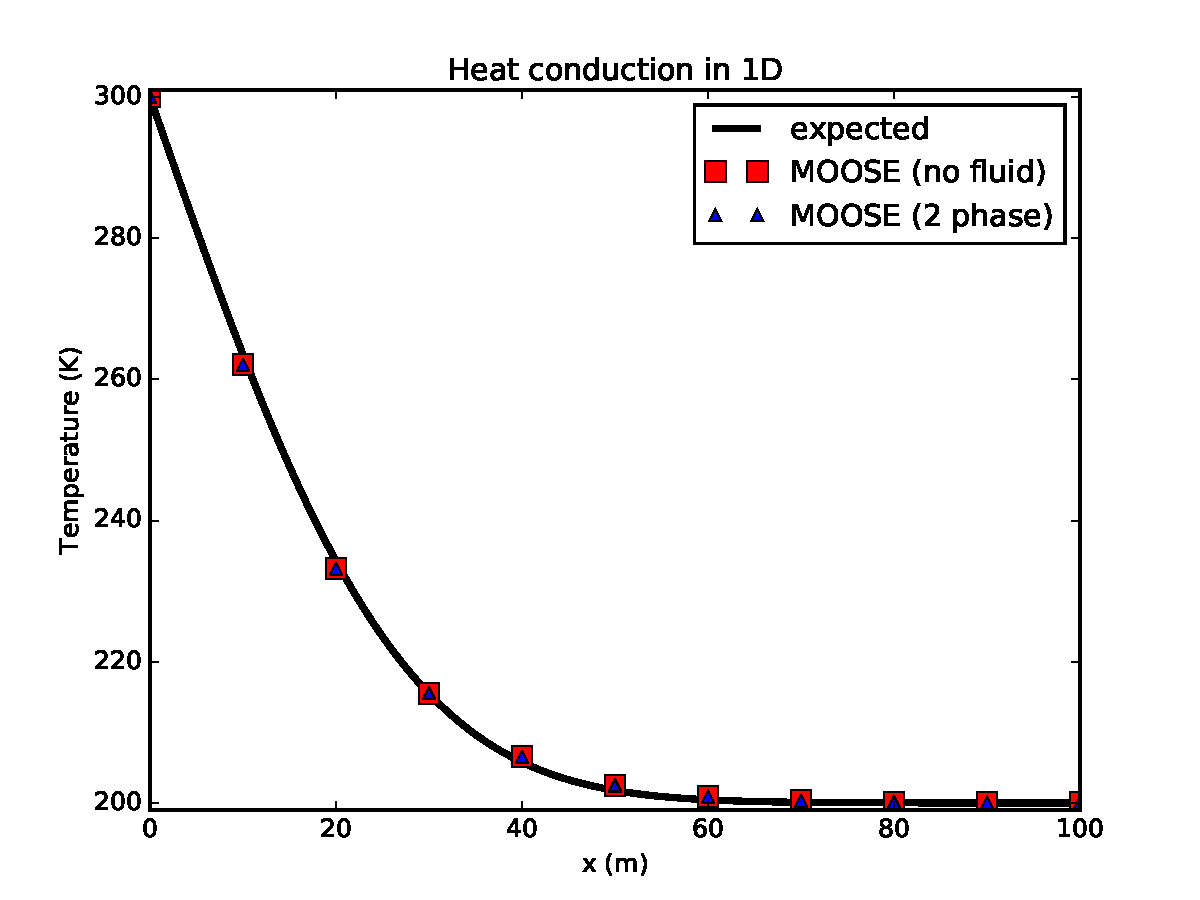
\includegraphics[width=15cm]{heat_conduction_1d.pdf}
\caption{Comparison between the MOOSE result (in dots), and the
  exact analytic expression given by Eqn~(\ref{eqn.exact.pp}).  This
  test had 10 elements in the $x$ direction, with $0\leq x \leq
  100$\,m, and ran for a total of
  10$^2$ seconds with 10 timesteps.}
\label{heat_conduction.fig}
\end{figure}



\end{document}

